\documentclass[border=4pt]{standalone}

\usepackage{tikz}

\def \setPSAT{ (0,-0.1) ellipse (25mm and 10mm) }
\def \setP{ (0,0) ellipse (8mm and 4mm) }
\def \setNP{ (-0.6,0) ellipse (15mm and 6mm) }
\def \setcoNP{ (0.6,0) ellipse (15mm and 6mm) }

\newcommand{\family}[1]
           {\ensuremath{\textnormal{\textsf{\textbf{#1}}}}}
\newcommand{\namedcollection}[1]
           {\ensuremath{\textnormal{\textsc{#1}}}}

\begin{document}
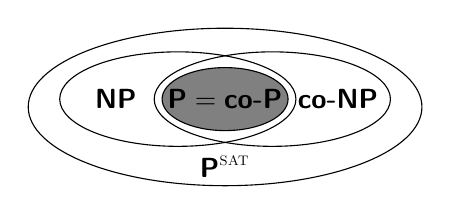
\begin{tikzpicture}

\filldraw[fill=gray] \setP node {$\family{P} = \family{co-P}$};
\draw \setNP node[left=4mm] {\family{NP}};
\draw \setcoNP node[right=2mm] {\family{co-NP}};
\draw \setPSAT node[below=5mm] {$\family{P}^\namedcollection{\tiny SAT}$};

\end{tikzpicture}
\end{document}